\begin{figure}[H]
  \begin{center}
    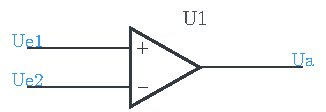
\includegraphics[width=0.618\textwidth]{circuits/komparator.pdf}
  \end{center}
  \caption{Einfache Komparatorschaltung}
\end{figure}

\[ U_a = V_0 (U_p - U_n) = V_0 (U_{e1} - U_{e2})\]

Ist $U_{e1}$ größer als $U_{e2}$ gerät der Operationsverstärker an seine
maximale positive Ausgangsspannung (idealerweise die
Versorgungsspannung), ist $U_{e1}$ kleiner als $U_{e2}$ an die maximal negative.
Legt man $U_{e2}$ auf einen konstanten positiven Referenzspannungswert, so verschiebt sich
die Kennline aus Abbildung 1 nach rechts.

\begin{figure}[H]
  \begin{center}
    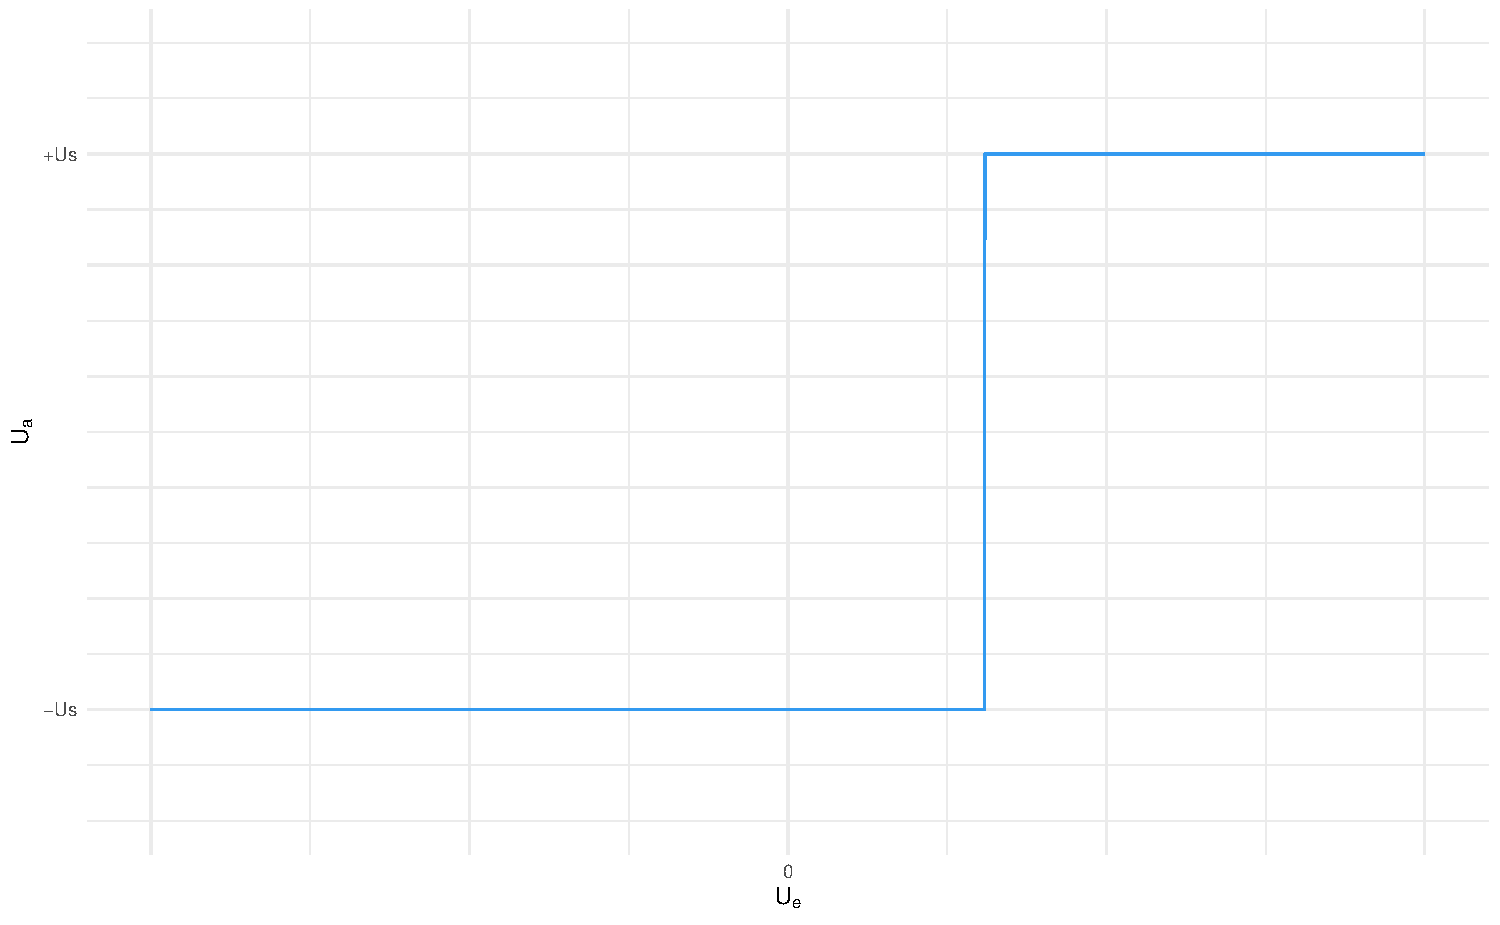
\includegraphics[width=\textwidth]{1_11/comparator.pdf}
  \end{center}
  \caption{Übertragungskennlinie der Komparatorschaltung mit positiver Referenzspannung ($U_{e2}$)}
\end{figure}


Zwischen invertierendem und nichtinvertierendem Eingang des
Operationsverstärkers können zwei Dioden antiparallel geschaltet werden, um die
Eingangsdifferenzspannung auf $\pm 0.7 \, \si{\volt}$ zu begrenzen. Zusätzlich
müssen dann zur Strombegrenzung Widerstände vor die Eingangs-/ Referenzspannung
geschaltet werden. 